% !TEX root=./report.tex

\subsection{Static calibration}

\ITS{} are inherently dependent on the calibration of the different sensors. 
To track and predict traffic the system has to know the poses of the different sensors relative to some reference coordinate system.
This enables the ITS to accurately measure the position of vehicles within the single sensor ranges and at the overlapping boundaries.

Previous experiments have shown that a calibration process based on an IMU is not feasible in our case. 
Instead we focus on a calibration procedure based on visual landmarks in the video feed.
The landmarks are mapped to their partially known world positions from high definition road maps. 

\paragraph{Retrive objects positions from the \HDmaps}
In this work we focus on the permanent delineator objects that are easily visible in the video feeds.

The world position of the objects can be retrieved using the mathematical operations defined in the \OD{} standard.

This gives us the the base origin point $o~=~(x, y, z)^T$ of the object in the transverse mercator projection \cite{proj}. 
The base origin point is the world position of the lower end of the object where it ends in the ground or another object.

Additionally we retrieve a directional heading axis $d~=~(x, y, z)^T$ and the height $h$ of the object.
\\
\\
These values enable us to approximate the real-world objects by sampling points $s \in S$ in world position 
along the center line of the object, where 
% \begin{equation}
%   S = \{(o + \lambda * d) : \lambda \in \Lambda \wedge \Lambda = \mathbb{R})\} \\
% \end{equation}

\begin{equation}
s = \{o, d, \lambda\} \in S, \quad \lambda \in \Lambda,  \quad \Lambda = \mathbb{R}
\end{equation}

and defines a world position calculated by

\begin{equation}
  w(s) = s_o + s_\lambda * s_d
  \end{equation}

\paragraph{Mapping pixels to objects}

To calibrate the camera we need to establish a mapping
\begin{equation}
  p_c \sim s_c
\end{equation}
from pixels $p_c~=~(u,v)^T \in P$ from the video stream to the corresponding sampled points $s_c$ from the object they belong to.

\begin{figure}[t]
  \begin{center}
  % \fbox{\rule{0pt}{2in} \rule{0.9\linewidth}{0pt}}
     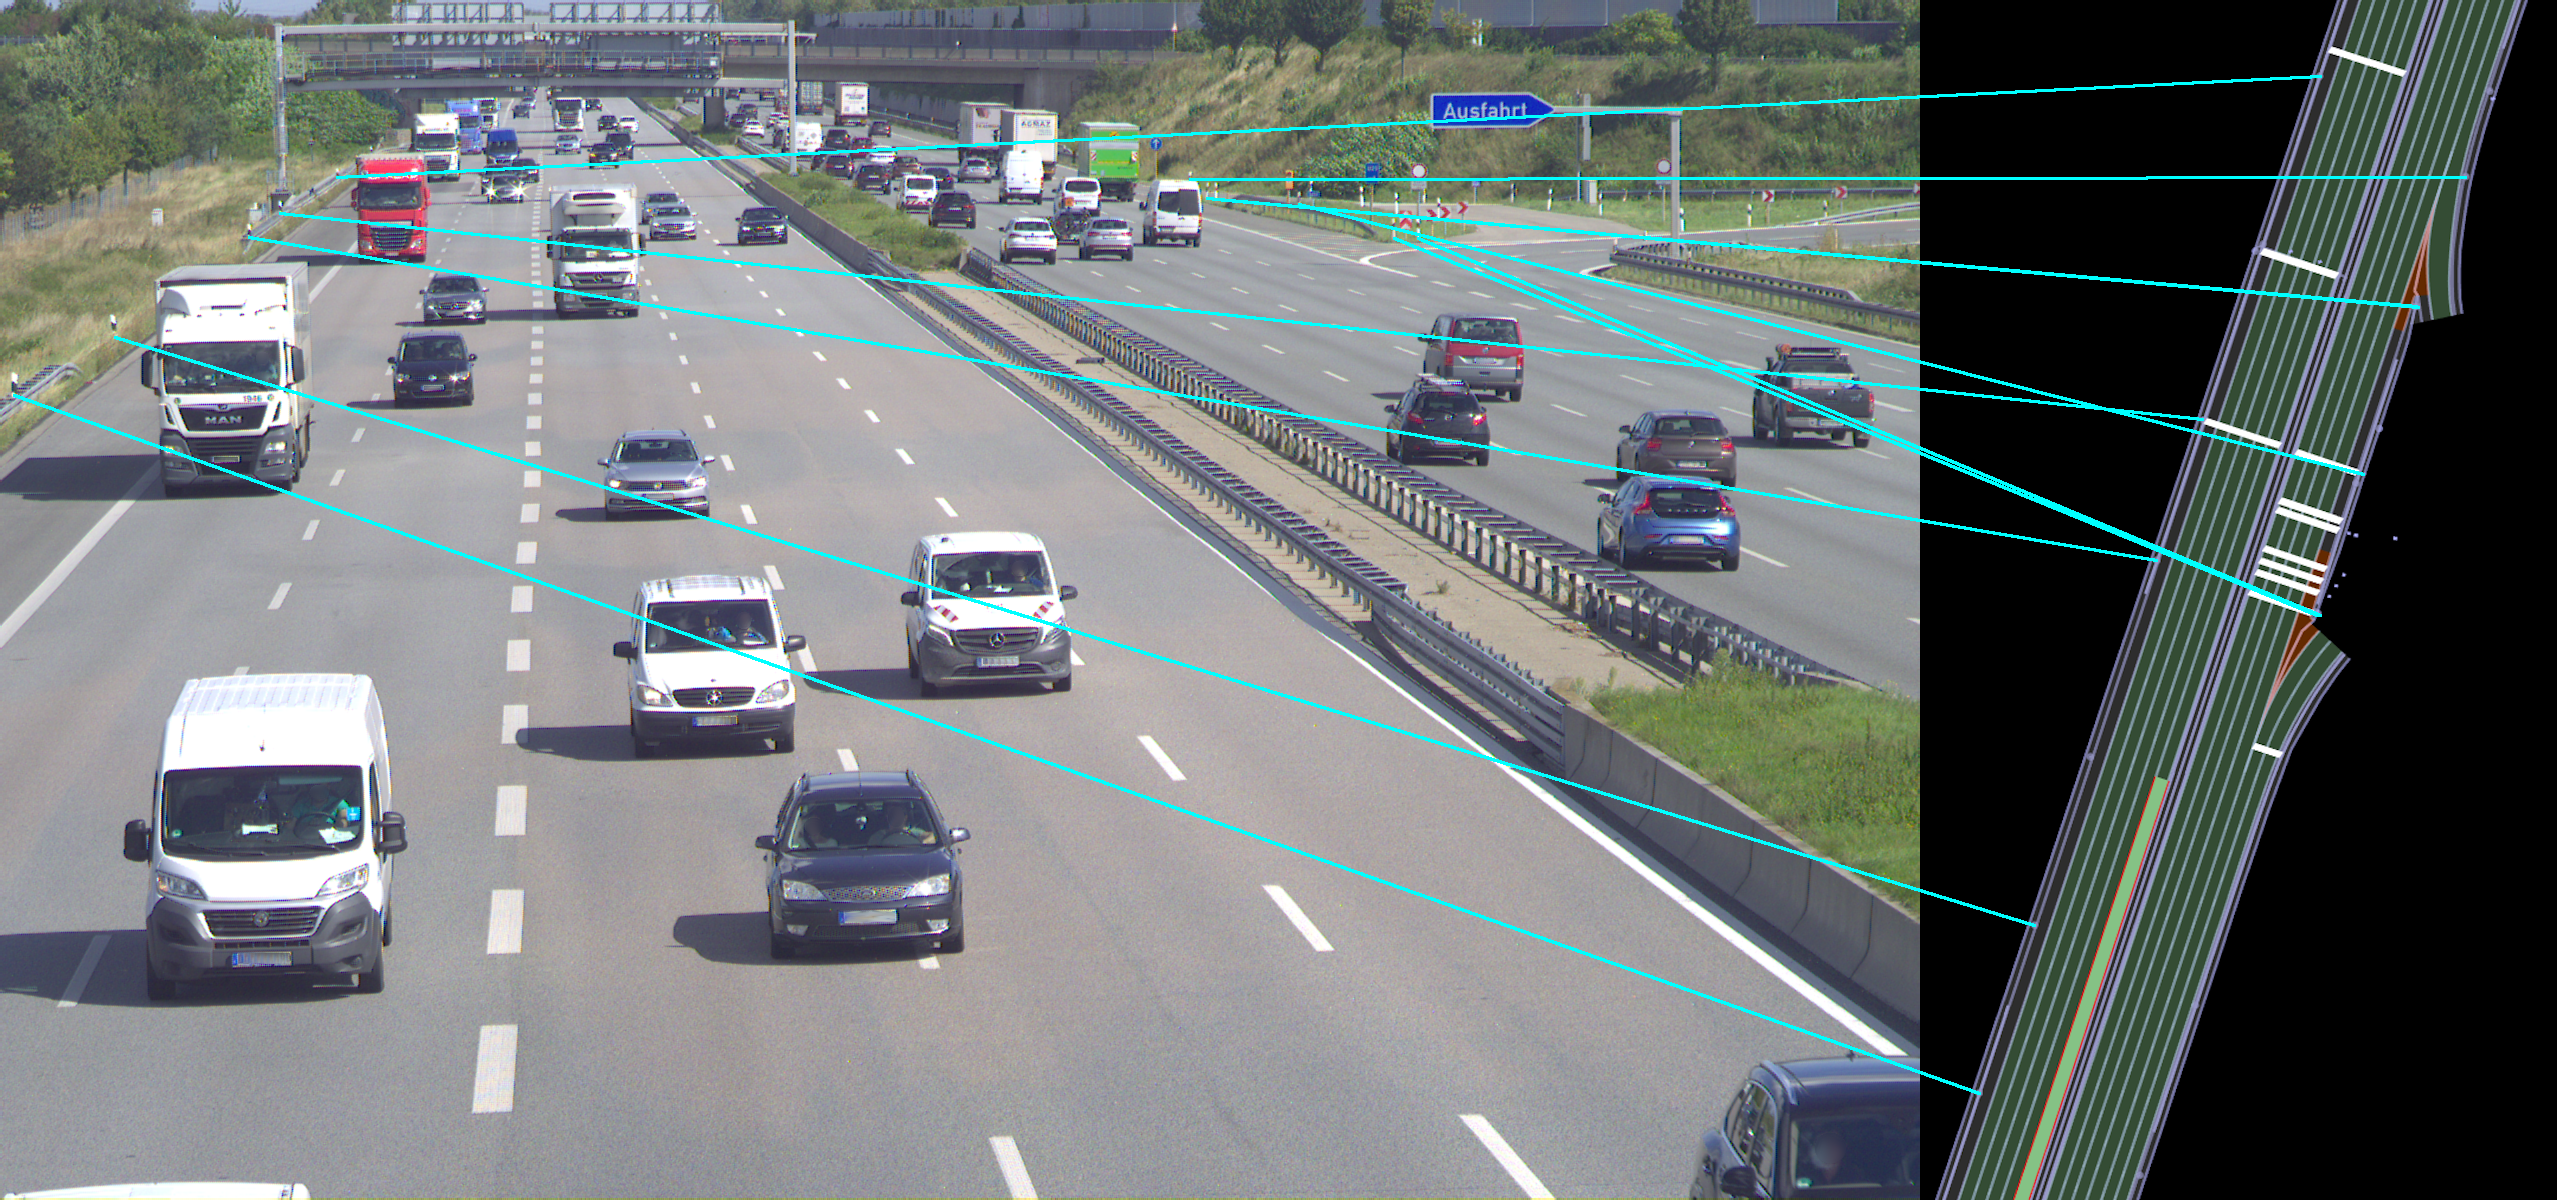
\includegraphics[width=\linewidth]{images/hd_map_mapping.png}
  \end{center}
     \caption{}
  \label{fig:hd_map_mapping}
  \end{figure}

\paragraph{Calibration procedure}

\begin{figure*}[t]
  \begin{tabular}{cc}
    \includegraphics[width=0.5\linewidth]{images/calibration/background_uncalibrated.png}    &  
    \includegraphics[width=0.5\linewidth]{images/calibration/background_calibrated.png}    
  \end{tabular}
  \caption{This is the calibration}
  \label{fig:calibration}
  \end{figure*}
  
Our camera is modelled using the pinhole camera model. 
This uses the known intrinsic camera parameters and their corresponding projection $\pi$ from camera to image space.

The extrinsic camera parameters that map from world space to camera space is defined by the camera translation $T$ and the camera rotation $R$.
The translation and rotation are unknown, for them we optimize. 

We estimate the camera pose by minimizing a modified version of the reprojection error 
\begin{equation}
  \min_{T, R, \Lambda} E(P, S, T, R, \Lambda) 
\end{equation}
formulated as
\begin{equation}
  \begin{split}
  E(P, S, T, R, \Lambda ) =& 
  \sum_{c} 
  \left\lVert 
  \begin{pmatrix}
    p_c - \pi(T * R * w(s_c))\\
    clamp(\lambda, 0, h)
  \end{pmatrix}
  \right\rVert_2^2 
\end{split}
\end{equation}

where $P$ is the set of mapped pixels in the image, $S$ is the set of mapped corresponding sampled points from the objects and $\Lambda$ is the set of $\lambda$ values associated with the sampled points and
\begin{equation}
    clamp(x, a, b) =
    \begin{cases}
      x - b,& \text{if } x > b\\
      x,    & \text{if } x < 0\\
      0,    & \text{else}
    \end{cases} 
\end{equation}

The world positions of the objects lie on the one-dimensional lines that approximate the objects we have to also optimize for the actual $\lambda$ values of the samples.
This jointly finds the world position of the samples and the pose of the camera.


% \begin{itemize}
%   \item HD map based approach
%   \item Optimization algorithm, reprojection error between map and video 
%   \item Landmark extraction, mapping, pose estimation
%   \item Watersheder for pixel marking
% \end{itemize}